In this section, we will develop the notation used for high-order matrix-free finite element operators.
The development of this notation will largely follow \cite{brown2010efficient}.

As mentioned in Section \ref{sec:highorderwhy}, finite element discretizations with tensor product bases offer performance on modern HPC software.
Therefore, this development will focus on arbitrary order tensor product bases, but this finite element operator representation does not depend upon the type of finite element.
Simplices or mixed finite element discretizations may be used with this finite element operator representation, although the choice of finite element bases will have performance implications.

Let $\lbrace X_i \rbrace_{i = 1}^p$ denote the Legendre-Gauss-Lobatto (LGL) nodes of degree $p - 1$ on the reference interval $\left[ -1, 1 \right]$ while $\lbrace \xi_i \rbrace_{i = 1}^q$ and $\lbrace w_i \rbrace_{i = 1}^q$ denote the quadrature points and quadrature weights corresponding to a $q$ point quadrature rule.
If we consider Lagrange basis functions $\lbrace \phi_i \rbrace_{i = 1}^p$, we can construct matrices $N_{i j} = \phi_j \left( \xi_i \right)$ and $D_{i j} = \partial_x \phi_j \left( \xi_i \right)$, representing interpolation of solution values to the quadrature points and computation of derivatives at the quadrature points, respectively.
Additionally, the quadrature weight matrix is given by $W_{i j} = w_i \delta_{i j}$.

We can define the corresponding matrices for problems in higher dimensions via tensor products.
For the specific case of 3D, we have
\begin{equation}
\begin{array}{c}
\mathbf{N}   = N \otimes N \otimes N \hspace{5mm}
\mathbf{D}_0 = D \otimes N \otimes N\\
\mathbf{D}_1 = N \otimes D \otimes N \hspace{5mm}
\mathbf{D}_2 = N \otimes N \otimes D\\
\mathbf{W}   = W \otimes W \otimes W
\end{array}
\label{eq:basis_ops}
\end{equation}
The basis operations in Equation \ref{eq:basis_ops} are defined on a reference element $\hat{K} = \left[ -1, 1 \right]^3$.

In finite element and spectral element methods, we partition the domain $\Omega$ into a set of $E$ elements, denoted $\lbrace K^e \rbrace_{e = 1}^E$ with coordinate mapping to the reference element given by $X : \hat{K} \rightarrow K^e$.
The Jacobian of this mapping is given by $J_{i j} = \partial x_i / \partial X_j$, where $X$ is the reference coordinates and $x$ the physical coordinates.
We can invert the Jacobian and compute the derivatives of the physical coordinates in the reference space at every quadrature point.
\begin{equation}
\mathbf{D}_i^e = \Lambda \left( \frac{\partial X_0}{\partial x_i} \right) \mathbf{D}_0 + \Lambda \left( \frac{\partial X_1}{\partial x_i} \right) \mathbf{D}_1 + \Lambda \left( \frac{\partial X_2}{\partial x_i} \right) \mathbf{D}_2
\end{equation}
where $\Lambda \left( X \right)_{i j} = X_i \delta_{i j}$ expresses pointwise multiplication of $J_{i j}^{-1}$ at quadrature points as a diagonal matrix.
With this coordinate mapping, element integration weights become $\mathbf{W}^e = W \Lambda \left( \lvert J^e \left( q \right) \rvert \right)$.

A global assembly operator is defined as $\mathcal{E}^T = \left[ \mathcal{E}^e \right]^T$, where $\mathcal{E}^e$ represents local restriction operators extracting degrees of freedom that correspond to element $e$ from the global solution vector.
When using an assembled matrix to represent a finite element operator, this global assembly operator is used to construct a global matrix representation of the finite element operator from the individual element operators.
With matrix-free implementations, this global assembly operator is instead used to assemble the action of the finite element operator on each element into the action of the finite element operator on the entire mesh.
Notice that the local restriction operators do not assume a structured mesh, a conforming mesh, or consistent polynomial order bases for each element.

With these definitions, we can represent the Galerkin system of equations corresponding to the weak form of arbitrary second order PDEs.
The weak form of PDEs is linear in test functions and can be expressed as pointwise operations where functions of $u$ and $\nabla u$ are contracted with $v$ and $\nabla v$.

Consider the weak form of an arbitrary PDE
\begin{equation}
\begin{array}{c}
\text{find } u \in V \text{ such that for all } v \in V\\
\langle v, u \rangle = \int_{\Omega} v \cdot f_0 \left( u, \nabla u \right) + \nabla v : f_1 \left( u, \nabla u \right) = 0
\end{array}
\label{eq:weak_form}
\end{equation}
where $\cdot$ represents contraction over fields and $:$ represents contraction over fields and spatial dimensions.
The pointwise representation of the weak form given by $f_0$ and $f_1$ does not depend upon discretization choices such as the geometry or polynomial degree of the bases.

The corresponding Galerkin system of equations is
\begin{equation}
\sum_e \mathcal{E}^T \left[ \left( \mathbf{N}^e \right)^T \mathbf{W}^e \Lambda \left( f_0 \left( u^e, \nabla u^e \right) \right) + \sum_{i = 0}^{d - 1} \left( \mathbf{D}_i^e \right)^T \mathbf{W}^e \Lambda \left( f_1 \left( u^e, \nabla u^e \right) \right) \right] = 0
\label{eq:galerkin_form}
\end{equation}
where $u^e = \mathbf{N}^e \mathcal{E}^e u$ and $\nabla u^e = \lbrace \mathbf{D}_i^e \mathcal{E}^e u \rbrace_{i = 0}^{d - 1}$.
In this formulation, the element restriction operators and basis operators can represent different element geometries and different degree polynomial bases, providing a flexible description for arbitrary meshes.
Furthermore, this notation can be extended to handle separate fields with different finite element bases, such as with mixed finite element methods.

Dirichlet boundary conditions are represented in the element restriction operation by enforcing the specified values on the constrained nodes.
Neumann or Robin boundary conditions are represented by adding boundary integral terms in the same form as Equation \ref{eq:galerkin_form} with appropriate basis and element restriction operators.
Boundary integrals internal to the domain $\Omega$, such as face integrals in Discontinuous Galerkin methods, can also be represented using additional terms with corresponding bases and element restrictions.

% -- Linearization ------------------------------------------------------------
\subsection{Linearization}

When the PDE in Equation \ref{eq:weak_form} is linear, the pointwise functions $f_0$ and $f_1$ are also linear and Krylov subspace methods can be used to solve the Galerkin system of equations in Equation \ref{eq:galerkin_form}.
When the PDE is non-linear, the Galerkin system in Equation \ref{eq:galerkin_form} provides the residual evaluator for a non-linear solver and Jacobian can be represented in a similar fashion as Equation \ref{eq:galerkin_form}, based upon the weak form
\begin{equation}
\langle v, J \left( u \right) w \rangle = \int_{\Omega}
\left[ \begin{array}{c c}
v^T & \left( \nabla v \right)^T
\end{array} \right]
\left[ \begin{array}{c c}
f_{0, 0} & f_{0, 1}\\
f_{1, 0} & f_{1, 1}
\end{array} \right]
\left[ \begin{array}{c}
w \\ \nabla w
\end{array} \right]
\label{eq:jacobian_form}
\end{equation}
where $f_{i, 0} = \frac{\partial f_i}{\partial u} \left( u, \nabla u \right)$ and $f_{i, 1} = \frac{\partial f_i}{\partial \nabla u} \left( u, \nabla u \right)$.
If these pointwise functions $f_{i, j}$ are not available analytically, they can be computed via algorithmic differentiation or finite differencing.

With these pointwise functions, we can describe Jacobian-free Newton-Krylov methods for solving non-linear PDEs.
Jacobian-free Newton-Krylov methods were summarized, with preconditioning strategies, by Knoll and Keyes in \cite{knoll2004jacobian}.

% -- Computational Representation ---------------------------------------------
\subsection{Computational Representation}

We can represent the systems of equations in Equation \ref{eq:galerkin_form} and Equation \ref{eq:jacobian_form} as a series of computational kernels, which may be fused in certain implementations.
This streamlined representation is used by libCEED \cite{libceed-user-manual} to provide performance portable implementations.
In Chapter \ref{ch:LocalFourierAnalysis}, we use this representation to develop LFA of high-order finite element operators and preconditioning methods.

The action of an arbitrary second-order finite element operator can be represented as
\begin{equation}
{\color{burgundy}\mathbf{A}} = \mathbf{P}^T \mathbf{G}^T {\color{blue(ncs)}\mathbf{B}}^T {\color{applegreen}\mathbf{D}} {\color{blue(ncs)}\mathbf{B}} \mathbf{G} \mathbf{P}
\label{eq:libceed_representation}
\end{equation}

where $\mathbf{P}$ represents the parallel communication portion of the global element restriction operator, $\mathbf{G}$ represents the device portion of the global element restriction operator, ${\color{blue(ncs)}\mathbf{B}}$ represents the basis action kernel that provides solution values and derivatives at the quadrature points, and ${\color{applegreen}\mathbf{D}}$ represents the pointwise representation of the weak form, given by $f_i$ or $f_{i, j}$ and the element quadrature weights and geometric factors.

\begin{figure}[ht!]
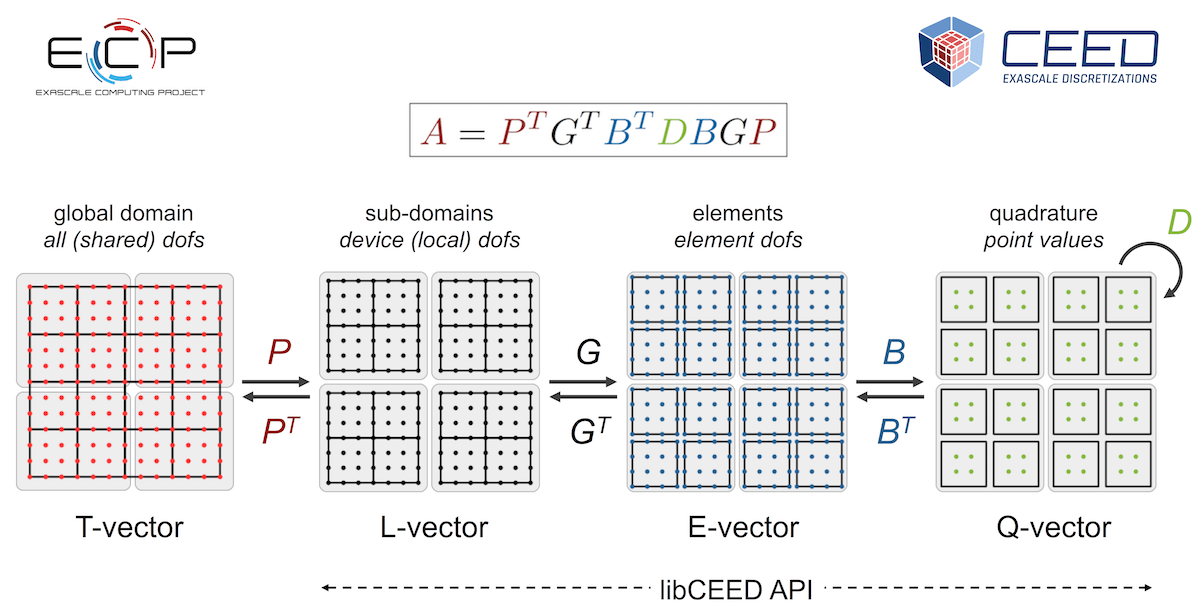
\includegraphics[width=.99\linewidth]{../img/libCEEDAPI}
\caption{libCEED API}
\label{fig:libceedapi}
\end{figure}

This representation is shown graphically in Figure \ref{fig:libceedapi}, where we can see the different spaces that each kernel operates upon.
These flexible kernels will be used in Chapter \ref{ch:SolidMechanics} in the implementation of the solid mechanics example for Neo-Hookean hyperelasticity at finite strain.
